\newcommand{\COMMENT}[1]{}

\section{An Informal Overview of \name} \label{sec:overview}

\name enriches a simple object-oriented language (supporting
parametric polymorphism and lambdas) with a set of region-specific
constructs.  In this section, we present an informal overview of these
region-specific constructs.

\subsection{Using Regions in \name}
\label{sec:alloc-ctxt}

\paragraph{Stack Regions} The ``\C{letregion R \{ S \}}'' construct
creates a new stack region, with a static identifier \C{R}, whose
scope is restricted to the statement \C{S}. The semantics of
\C{letregion} is similar to Tofte and Talpin~\cite{tofte94}'s
\C{letregion} expression: objects can be allocated by \C{S} in the
newly created region while \C{R} is in scope, but the region and all
objects allocated within it are freed at the end of \C{S}.

\paragraph{Object Allocation} The ``\C{new@R T()}'' construct creates
a new object of type \C{T} in the region \C{R}. The specification of
the allocation region \C{R} in this construct is optional.  At
runtime, \name maintains a stack of \emph{active} regions, and we
refer to the region at the top of the stack as the \emph{allocation
context}. The statement \C{new T()} allocates the newly created object
in the current allocation context.
%
This is important as it enables \name applications to use existing
region-oblivious C\# libraries. In particular, given a  C\# library
function \C{f} (that makes no use of \name's region constructs), the
statement ``\C{letregion R \{ f(); \}}'' invokes \C{f}, but has the
effect that all objects allocated by this invocation are allocated in
the new region \C{R}.

\paragraph{Transferable Regions} \name's \emph{transferable regions}
are an encapsulation of a data-structure that can be transferred
between autonomous entities (\eg, between two concurrently executing
threads or actors).  Hence, unlike stack regions, transferable regions
are not constrained to have a lexically scoped lifetime.  (Hence, we
also refer to them as \emph{dynamic} regions.)

Furthermore, transferable regions, unlike stack regions, are first
class values of \name: they are objects of the class \C{Region}, they
are created using the \C{new} keyword, and can be passed as arguments,
stored in data structures, and returned from methods.  A transferable
region is intended to encapsulate a single data-structure, consisting
of a collection of objects with a distinguished root object of some
type \C{T}, which we refer to as the region's \emph{root} object.  The
class \C{Region} is parametric over the type \C{T} of this root
object.

The \C{Region} constructor takes as a parameter a function that
constructs the root object: it creates a new region and invokes this
function, with the new region as the allocation context, to create the
root object of the region. The following code illustrates the
creation of a transferable region, whose root is an object of type
\C{A}.
% (\C{r}) of type \C{T}:
\begin{codejava} 
  Region<A> rgn = new Region<T>(() => new A())
\end{codejava} 
In the above code, \C{rgn} is called the \emph{handler} to the newly
created region, and is required to read the contents of the region, or
change its state. The class \C{Region} offers two methods: a \C{free}
method that deallocates the region (and all the objects allocated
within it), and \C{transfer} method that transfers the region to a
consumer process. It is an abstraction of two possible forms of
transfer: a transfer between two processes in a shared memory setting
or a transfer between two processes in a distributed, message-passing,
setting. The precise semantics of \C{transfer} are unimportant in the
context of the region type system and we will not discuss them
further. \dv{this is a bit counter-intuitive.} 

% \begin{figure} \begin{codejava} public class Region<T> { public
% Region(Func<T> mkRoot); public void free(); public void transfer();
% } \end{codejava} \caption{The type signature of the \C{Region}
% class} \label{fig:region-class} \end{figure}

% The type signature of the class \C{Region} appears in
% Fig.~\ref{fig:region-class}.  The method \C{free} deallocates the
% region (including all objects allocated within it).  The method
% \C{transfer} transfers the region to a downstream actor as
% determined by the run-time.  It is an abstraction of two possible
% forms of  transfer: a transfer between two actors in a shared memory
% setting or a transfer between two actors in a distributed,
% message-passing, setting.  The precise semantics of \C{transfer} are
% unimportant in the context of the region type system and we will not
% discuss them further.

\paragraph{Open and Closed Regions} A transferable region must be
explicitly \emph{opened} using \name's \C{open} construct in order to
either read or update or allocate objects in the region.
Specifically, the construct ``\C{open rgn as v@R \{ S \}}'' does the
following: (a). It opens the transferable region handled by \C{rgn}
for allocation (i.e., makes it the current allocation context), (b).
binds the identifier \C{R} to this open region, and (c). initializes
the newly introduced local variable \C{v} to refer to the root object
of the region.  The \C{@R} part of the statement is optional and may
be omitted.  The \C{open} construct is intended to simplify the
problem of ensuring memory safety, as will be explained soon.  We
refer to a transferable region that has not been opened as a
\emph{closed} region.

\paragraph{Motivating Example}
% We now illustrate how the features of \name can be used to 
Fig.~\ref{fig:motivating-eg-in-broom} shows how the motivating example
of Fig.~\ref{fig:motivating-eg} can be written in \name.  The
\C{onReceive} method receives its input message in a
\emph{transferred} region (\ie, a \emph{closed} region whose ownership
is transferred to the recipient).  Line 7 creates a new region to
store the output for time \C{t}, initializing it to contain an empty
list.  Line 9 opens the input region to process it\footnote{We omit
\C{@R} annotation in \C{open} when we don't need \C{R}.}.  Line 10
creates a stack region \C{R0}.  Thus, the temporary objects created by
the iteration in line 11, for example, will be allocated in this stack
region that lives just long enough.  We open the desired output region
in line 12, so that the new output objects created by the invocation
of \C{selector} in line 13 are allocated in the output region.
Finally, the input region is freed in line 15. The output region at
\C{map[t]} stays as along as input messages with timestamp \C{t} keep
arriving. When the timing message for \C{t} arrives, the \C{onNotify}
method transfers the \C{outRgn} at \C{map[t]} to a downstream actor.
% After the transfer, \C{SelectVertex} is no longer allowed to access
% the \C{outRgn}, facilitating its deallocation.

\begin{figure}[t!]
\begin{numcodejava}
class SelectVertex<TIn, TOut> {
  Func<TIn, TOut> selector;
  Dictionary<Time, Region<List<TOut>>> map;
  ...
  void onReceive(Time t,Region<List<TIn>> inRgn){
    if (!map.ContainsKey(t))
       map[t] = new Region<List<TOut>> (
                  () => new List<TOut>());
    open inRgn as inputList {
      letregion R0 {
        foreach (TIn input in inputList) {
          open map[t] as outRgn {
            TOut output = selector(input);
            outRgn.add(output); } } } }
    inRgn.free();
  }
  void onNotify(Time t) {
     Region<List<TOut>> outRgn = map[t];
     map.Remove(t);
     outRgn.transfer();
  }
}
\end{numcodejava}
\caption{\C{SELECT} dataflow operator in \name}
\label{fig:motivating-eg-in-broom}
\vspace*{-0.15in}
\end{figure}


\subsection{Memory Safety} \label{sec:memory-safety}

Our goal is a type system that can ensure the memory safety of
programs that use the region constructs described above.  The key to
memory safety in \name is the following restriction: an object $o_1$
in a region $R_1$ is allowed to store a pointer to an object $o_2$ in
a region $R_2$ only if $R_2$ is guaranteed to outlive $R_1$.  (A
similar restriction applies in the case where $o_1$ is a
stack-allocated variable.)

Enforcing this restriction is simple in the case of stack regions
since the outlives relation between stack regions can be inferred from
their lexical nesting. Unfortunately, inferring outlives relations
in presence of transferable regions is not easy.  \name imposes the following
protocol on the use of transferable regions to help simplify this
check.

A transferable region (that has not been freed or transferred) can be
in one of two possible states, \emph{open} or \emph{closed}. A newly
created region is in the closed state.  A region must be opened, using
the open construct (as explained previously), in order to read or
update or allocate an object within that region.  An open region
cannot be freed or transferred.  In particular, an open region is
guaranteed to be live for the entire duration of the open construct.
This allows the type system to infer a valid outlives relation between
the opened region and any stack region that is nested within the open
construct.

\begin{figure} 
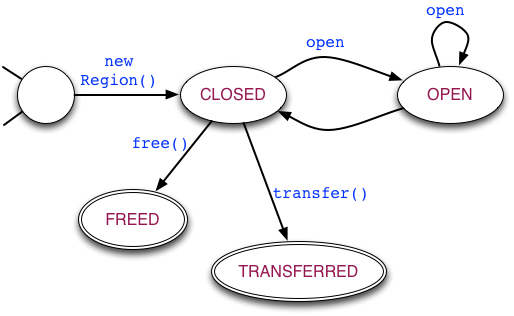
\includegraphics[scale=0.45]{region-fsm.png}
\caption{The lifetime of a dynamic (transferable) region in \name}
\label{fig:region-fsm} 
\vspace*{-0.25in} 
\end{figure}

The protocol for transferable regions is presented as a finite state
machine in Fig.~\ref{fig:region-fsm}.  
% A transferable region starts
% its lifetime in a \emph{closed} state, when it is created.
%
The safety of memory accesses in \name is now subject to the condition
that every transferable region correctly follows the state transition
discipline of Fig.~\ref{fig:region-fsm}. Under this condition, \name's
region type system statically guarantees the safety of all memory
accesses.
% In other words, the type system reduces the problem of ensuring
% memory safety in \name programs to the problem of enforcing the
% state transition discipline for transferable regions.

In \name, this enforcement is done at runtime by explicitly keeping
track of the \emph{current state} for $\RgnZ$ objects, and checking
the validity of every open, transfer, or free operation and throwing
an exception if it is invalid.  
% The challenge in enforcing this
% discipline statically is that transferable regions are first-class
% objects. Hence, the program can create multiple aliases for the same
% region, \eg, open it via one alias and free it via another.  Typestate
% verification in the presence of aliases is hard.  The checking can be
% done statically by preventing the creation of aliases using, \eg,
% linear types or unique types. However, this would be quite
% restrictive, in terms of expressiveness.
As explained previously, this is a reasonable trade-off in the context
of \name, as regions are coarse-grained objects, which are manipulated
infrequently, when compared to fine-grained objects that reside inside
these regions. Therefore, runtime overhead of checking the region's
state transition discipline is acceptable.

\begin{figure*}[t!]
%
\begin{smathpar}
\renewcommand{\arraystretch}{1.2}
\begin{array}{lclcl} 
\multicolumn{5}{c}{
  {\rgn} \in \mathtt{Static \; region \; ids} \qquad
  {\rho} \in \mathtt{Region \; variables} \qquad
  {\tyvar, \tyvarb} \in \mathtt{Type \; variables} \qquad
  {m} \in \mathtt{Method \; names} \qquad
  {x,y,f} \in \mathtt{Variables \; and \; fields} }\\
cn & \in & \M{Class \; names} & \coloneqq & \ObjZ \ALT \RgnZ \ALT A \ALT B\\
     \fgjN & \in & \M{FGJ \; class \; types} & \coloneqq & cn\inang{\tbar}\\
T  & \in & \M{FGJ \; types} & \coloneqq & \tyvar \ALT  \fgjN \ALT \unitZ
     \ALT \bar{T} \rightarrow T \\
\fbN  & \in & \M{Region-annotated \; class \; types} & \coloneqq & 
     cn\inang{\tbar}\inang{\rbar} \\
\tau &\in& \M{types} & \coloneqq & T@\rgn  
      \ALT \fbN \ALT \unitZ 
      \ALT \inang{\rhobar \,|\, \phi}\bar{\tau}
      \xrightarrow{\rgn} \tau \\
C  & \in & \M{Class \; definitions} & \coloneqq & 
     \C{class} \; cn\inang{\bar{\tyvar} \extends \bar{\fgjN}} 
                    \inang{\rhobar \,|\, \phi}\extends \fbN 
                    \{\bar{\tau} \; \bar{f};\; \bar{d}\}\;\\
%k  & \in & \M{Constructors} & \coloneqq & 
%     cn(\bar{\tau} \; \bar{x})\{\C{super}(\bar{x}); \;
%                                \C{this}.\bar{f}\,=\,\bar{x};\}\\
d  & \in & \M{Methods} & \coloneqq & 
     \tau \; m\inang{\rhobar \,|\, \phi} (\taubar \; \xbar)
     \{\C{return}\;e;\}\\
\phi,\phicx &\in& \M{Region\;constraints} & \coloneqq & true 
      \ALT \rho \outlives \rho \ALT \rho = \rho \ALT \phi \conj \phi\\
e  & \in & \M{Expressions} & \coloneqq & \unitval \ALT x \ALT e.f 
     \ALT e.m\inang{\rbar}(\ebar) \ALT \C{new}\;\fbN(\ebar)
     \ALT \lambdaexp{\rgn}{\rhobar \,|\, \phi}
                    {\xbar:\taubar} {e}
           \ALT e\inang{\rbar}(\bar{e})\\
   & & & & \ALT \letexp{x}{e}{e} \ALT \letregion{\rho}{e} 
           \ALT \open{x}{\rgn}{y}{e} \\
\end{array}
\end{smathpar}

\caption{\fbname: Syntax}
\label{fig:fb-syntax}
\end{figure*}


\paragraph{Cloning} Note that in the example from
Fig.~\ref{fig:motivating-eg-in-broom} the object returned by the
\C{selector} (on Line 13) should not contain any references to the
input object, since the input region, where the object resides, will
be freed at the end of the method. If there is a need for the output
object to point to subobjects of the input object, such subobjects
must be cloned (to copy them from the input region to the output
region).  Fortunately, \name's region type system
(\S~\ref{sec:type-system}) is capable of capturing such nuances in the
type of \C{selector} and the type checker will ensure correctness.
Furthermore, the type can be automatically inferred by \name's region
type inference (\S~\ref{sec:type-inference}), which can perform the
above reasoning on behalf of the programmer.


%\begin{codejava} Region<string> rgn = new Region<List<String>> (() =>
%new List<String>()); open rgn as  strList@R0 {
%strList.addAtHead("World"); strList.addAtHead("Hello"); }
%rgn.transfer(); \end{codejava}

\COMMENT{ \subsection{Stack Regions and Outlives Relation}

The \C{letregion} blocks can be nested, leading to a stack of regions
that are deallocated in the reverse order in which they are allocated.
Following ~\cite{cyclonepldi02}, we therefore call regions introduced
by \C{letregion} expressions as \emph{stack regions}. The stack
discipline induces an \emph{outlives} relationship among regions
created by nested \C{letregion}s, where the region introduced by the
outer \C{letregion} is guaranteed to outlive the one introduced by the
inner \C{letregion}. It is therefore safe to refer to an object
allocated in outer region from the inner region, but the converse is
not true. For example, consider the following code (assume that class
\C{A} has field \C{x} of type \C{Object}): \begin{center}
\begin{codejava} letregion R0 { A a0 = new@R0 A(); letregion R1 { A a1
= new@R1 A(); a1.x = new@R0 Object(); // safe & legal a0.x = new@R1
Object(); // unsafe & illegal ...  } ...  } \end{codejava}
\end{center} The code creates two stack regions with identifiers
\C{R0} and \C{R1}, where the region \C{R0} outlives the region \C{R1}
(denoted as $\C{R0} \outlives \C{R1}$).  Objects \C{a0} and \C{a1} are
allocated in regions \C{R0} and \C{R1}, respectively. The first
assignment statement assigns to \C{a1.x} an object allocated in outer
region (\C{R0}). This assignment is safe as \C{a1.x} refers to a
longer living object, hence is guaranteed to be a valid reference
throughout the lifetime of \C{a1}.  In contrast, the second assignment
is unsafe, as it assigns to \C{a0.x} an object, whose lifetime is
shorter than the lifetime of \C{a0}, making it unsafe to dereference
\C{a0.x} outside the inner block. 
% Unsafe assignments can also happen indirectly via a function call..
Preempting such unsafe assignments is the \emph{raison d'etre} of the
region type system.

\subsection{Allocation Context and Qualified Region Polymorphism}
\label{sec:alloc-ctxt}

Observe that \C{listIterator} can be called under multiple different
allocation contexts, and each time it returns a \C{ListIterator}
allocated in its allocation context. The iterator object might hold
references to the list, requiring the list to be allocated in a region
that outlives \C{listIterator}\!'s allocation context. However, modulo
this constraint, \C{listIterator} is not concerned about where the
list is allocated. As such, \C{listIterator} is
\emph{region-polymorphic} with respect to (a). its allocation context
argument, and (b). the allocation region of the list, subject to the
constraint that the later outlives the former. We call such region
polymorphism with constraints in \name as \emph{qualified region
polymorphism}. The provision to elide allocation region
specifications, and the ability to infer qualified region-region
polymorphic types are pivotal to interface region-oblivious standard
library code with region-aware application code in \name. 

\subsection{Dynamic (Transferable) Regions}



In a typical dataflow computation, an upstream actor (e.g., a
\C{SELECT} operator) constructs a transferable region, sets its root
to the data structure containing intermediate results, and then
transfers it to a downstream actor (e.g., a \C{COUNT} operator), which
performs further processing. Since a transferable region escapes the
lifetime of the sender, there must be no references from inside of the
transferable region to objects allocated in other memory regions of
the sender. Such references, if exist, may become invalid references
in the context of recipient's address space, jeopardizing memory
safety. \name relies on its region type system to prevent such unsafe
references from being created.

%% USING TEMPORARY STACK REGIONS AND ITS CORRECTNESS

\name lets stack regions to be used as working memory while operating
with the data stored in a transferable region. Consider the following
code, for instance\footnote{For brevity, we drop the region identifier
binding part of the \C{open} expression whenever the identifier is not
used.}: \begin{codejava} void onReceive(Region<List<String>> rgn) open
rgn as strList { letregion R1 { String s = ""; ListIterator<String> i
= strList.listIterator(); while(i.hasNext()) { s += i.getNext(); }
print s; //prints "HelloWorld" } } rgn.free(); \end{codejava} The
stack region \C{R1} is being used in the above code to provide working
memory to work with the objects of transferable region \C{rgn}. Since
a transferable region cannot be transferred/freed while it is still
open (Fig~\ref{fig:region-fsm}), \C{rgn} is guaranteed to outlive the
stack region \C{R1} in the above code, making it safe for the later to
contain references to the former. \name therefore allows such
references.

As Fig.~\ref{fig:region-fsm} indicates, it is not possible to open a
region that is already transferred/freed. The fact that \C{rgn} is
open within the block therefore guarantees that it is not yet
transferred/freed, and that dereferencing \C{strList} within the block
is safe. The end of \C{open} block marks the return of transferable
region to the closed state.  While closed, the region is eligible to
be transferred to a downstream actor, or to be freed.  An actor that
receives the transferable region, receives it in the closed state. It
can then reopen the received region to read its contents, possibly add
more data and transfer it to another actor, or free the region. 

}

